\documentclass{standalone}
\usepackage{../../../../preamble_formulas}

\begin{document}
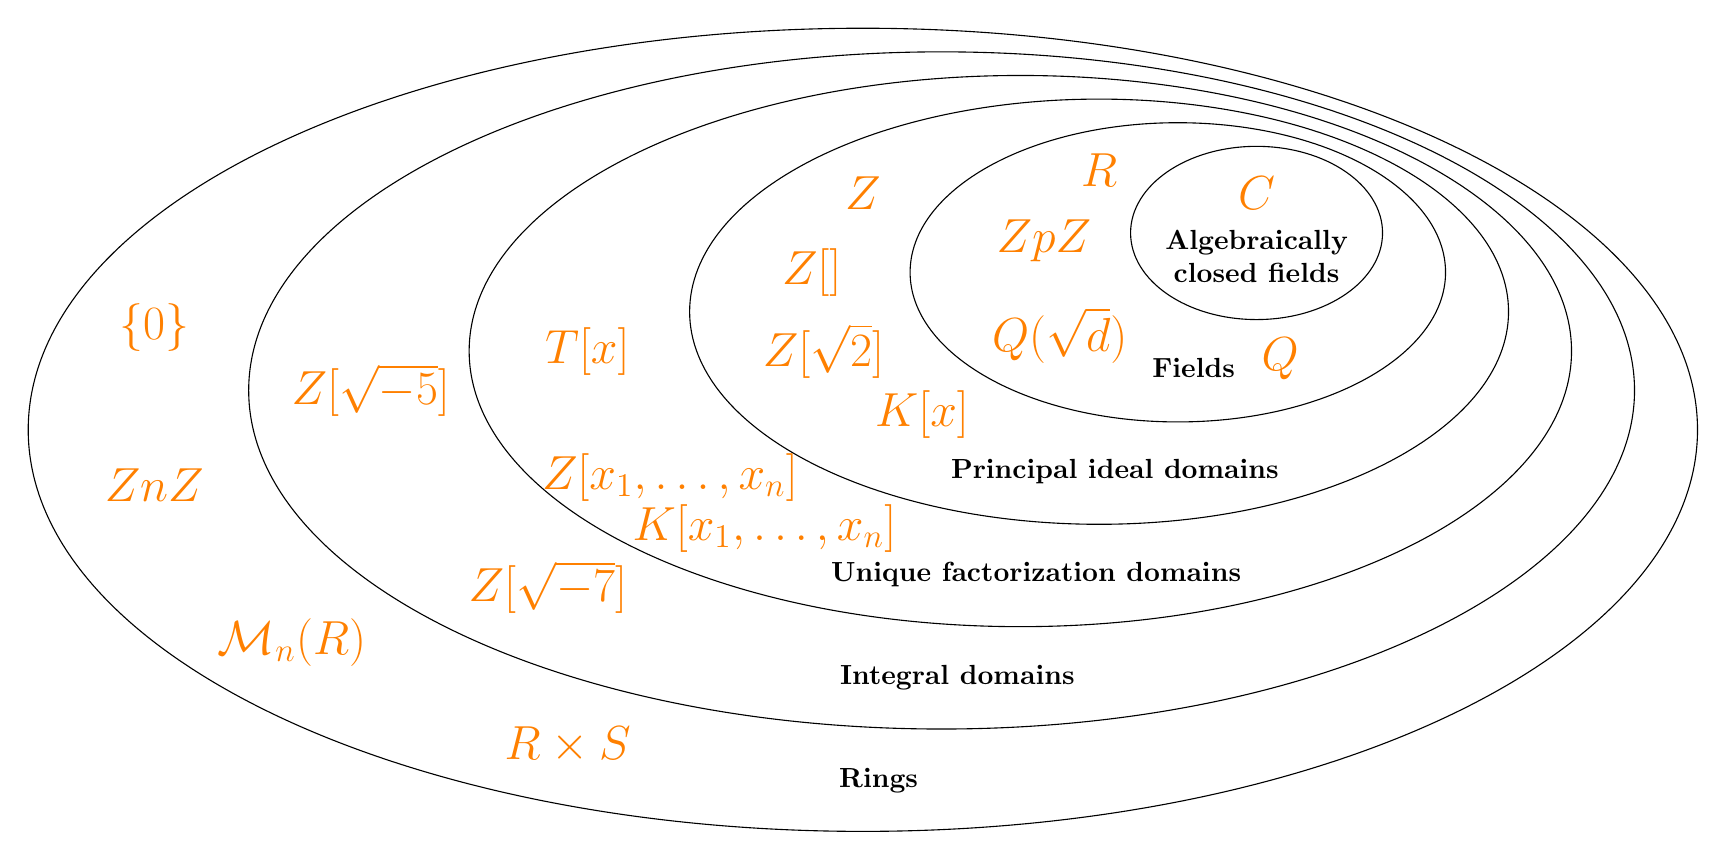
\begin{tikzpicture}
    \node[align=center,font=\bf] at (-1,-0.8) {Algebraically\\closed fields};
    \foreach \X [count=\Y starting from 1.5] in {,Fields,Principal ideal domains,Unique factorization domains,Integral domains,Rings}
        {\draw (-\Y,-\Y/2) ellipse ({1.8*\Y-0.2} and 0.8*\Y+0.3);
            \node[font=\bf] at (-\Y+0.2,-1.31*\Y+0.4) {\X}; }

    \node[color=orange] at (-15,-1.7) {\LARGE $\{0\}$}; %R
    \node[color=orange] at (-15,-3.7) {\LARGE $\displaystyle\quot{\mathbb{Z}}{n\mathbb{Z}}$}; %R
    \node[color=orange] at (-13.25,-5.7) {\LARGE $\mathcal{M}_n(R)$}; %R
    \node[color=orange] at (-9.75,-7) {\LARGE $R\times S$}; %R
    \node[color=orange] at (-12.25,-2.5) {\LARGE $\mathbb{Z}[\sqrt{-5}]$}; %ID.
    \node[color=orange] at (-10,-5) {\LARGE $\mathbb{Z}[\sqrt{-7}]$}; %ID.
    \node[color=orange] at (-9.5,-2) {\LARGE $T[x]$}; %UFD
    \node[color=orange,rotate=0] at (-8.45,-3.6) {\LARGE $\mathbb{Z}[x_1,\ldots,x_n]$}; %UFD
    \node[color=orange,rotate=0] at (-7.25,-4.25) {\LARGE $K[x_1,\ldots,x_n]$}; %UFD
    \node[color=orange] at (-6,0) {\LARGE $\mathbb{Z}$}; %PID
    \node[color=orange] at (-6.65,-1) {\LARGE $\mathbb{Z}[\ii]$}; %PID
    \node[color=orange] at (-6.5,-2) {\LARGE $\mathbb{Z}[\sqrt{2}]$}; %PID
    \node[color=orange] at (-5.25,-2.8) {\LARGE $K[x]$}; %PID
    \node[color=orange] at (-3.7,-0.6) {\LARGE $\displaystyle\quot{\mathbb{Z}}{p\mathbb{Z}}$}; %F
    \node[color=orange] at (-3,0.3) {\LARGE $\mathbb{R}$}; %F
    \node[color=orange] at (-0.7,-2.1) {\LARGE $\mathbb{Q}$}; %F
    \node[color=orange] at (-3.5,-1.8) {\LARGE $\mathbb{Q}(\sqrt{d})$}; %F
    \node[color=orange] at (-1,0) {\LARGE $\mathbb{C}$}; %ACF
\end{tikzpicture}
\end{document}